\chapter{Budowa dwukołowego robota balansującego}
\label{chap:budowa}

W celu przetestowania zaimplementowanych metod fuzji sygnałów pochodzących z czujnika ruchu, oraz algorytmu sterowania opartego na dwóch regulatorach PID połączonych kaskadowo, powstał rzeczywisty model robota balansującego. Jednym z założeń realizacji projektu było wykorzystanie gotowych modułów elektronicznych, tak aby zaoszczędzić czas podczas wykonywania konstrukcji oraz umożliwić ich łatwą ewentualną wymianę w celu naprawy, lub wykorzystania w innych projektach. Do wykonania konstrukcji użyto:
\begin{itemize}
    \item zaprojektowany w SolidWorksie korpus wycinany laserowo z płyty pleksi
    \item dwustronną płytkę PCB wykonana domową metodą termotransferu
    \item dwa koła o średnicy ok. 8 cm z mocowaniami wykonanymi własnoręcznie ze stalowych pięciokątnych słupków dystansowych
    \item dwa sterowniki Pololu A4988 RepRap 35V/2A
    \item baterię LiPo 11.1V / 1300mAh
    \item dwa silniki krokowe JK42HS48-1684 200 kroków/obr 2.8V / 1.68A / 0.43Nm
    \item płytkę z mikrokontrolerem Nucleo F103RB
    \item moduł bluetooth HC-05
    \item dwie regulowane przetwornice impulsowe step-down LM2596 3.2V-35V / 3A
\end{itemize}

Do obsługi modułów, potrzebne były takie peryferia jak $I^2C$, UART oraz PWM. Idea obsługi najważniejszych modułów przez poszczególne peryferia mikrokontrolera przedstawiona została na rysunku \ref{Moduly}

\begin{figure}[h!]
    \centering
    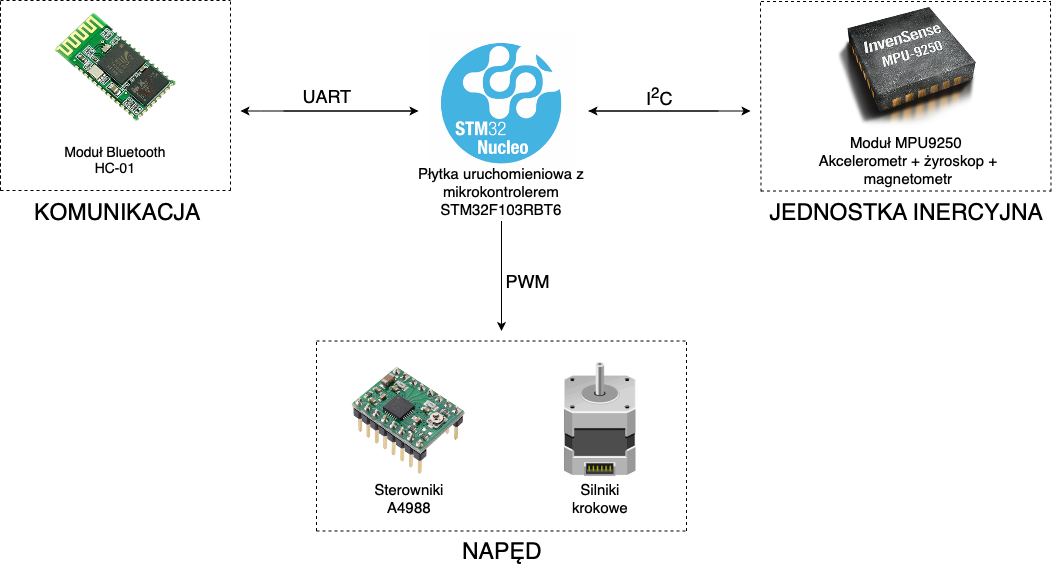
\includegraphics[width=1\textwidth]{Rysunki/Rozdzial05/Platforma_sprzetowa.png}
    \caption{Wykorzystane w budowie moduły}
    \label{Moduly}
\end{figure}

%----------------------------------------------------------------------------------------------------------------
\section{Konstrukcja mechaniczna}

Budowę robota, rozpoczęto od fazy koncepcyjnej, w której zaplanowano rozmieszczenie poszczególnych elementów, które można zobaczyć na rysunku \ref{Faza koncepcyjna}.

\begin{figure}[h!]
    \centering
    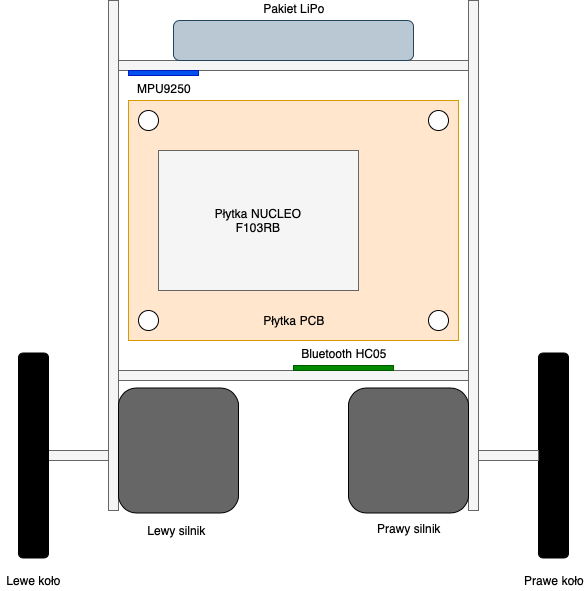
\includegraphics[width=0.5\textwidth]{Rysunki/Rozdzial05/Faza_koncepcyjna.png}
    \caption{Rozmieszczenie elementów}
    \label{Faza koncepcyjna}
\end{figure}

Kolejnym etapem, było zaprojektowanie korpusu, który zdecydowano się wykonać z poliwęglanu o grubości 5mm, ze względu na łatwą dostępność i stosunkowo niski koszt. Projekt został wykonany w programie \texttt{SolidWorks}, a rama została wykonana na zamówienie w firmie oferującej usługi laserowej obróbki poliwęglanu, na podstawie rysunków wykonawczych przedstawionych na schemacie \ref{rysunki wykonawcze}. Wyrenderowana rama robota została zaprezentowana na rysunku \ref{render}.

\begin{figure}[h!]
    \centering
    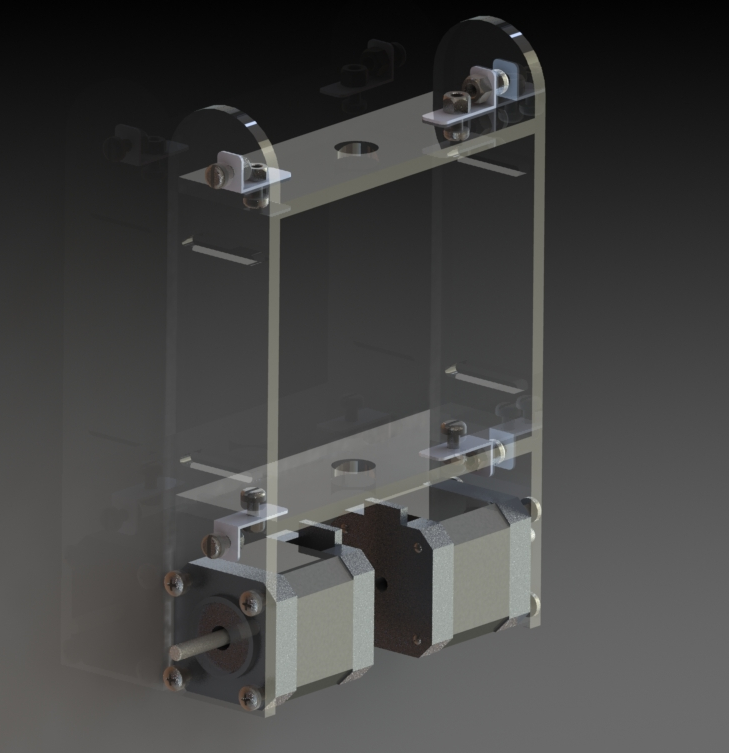
\includegraphics[width=0.5\textwidth]{Rysunki/Rozdzial05/rama.png}
    \caption{Wyrenderowany wygląd zaprojektowanego korpusu}
    \label{render}
\end{figure}

\begin{figure}[h!]
    \centering
    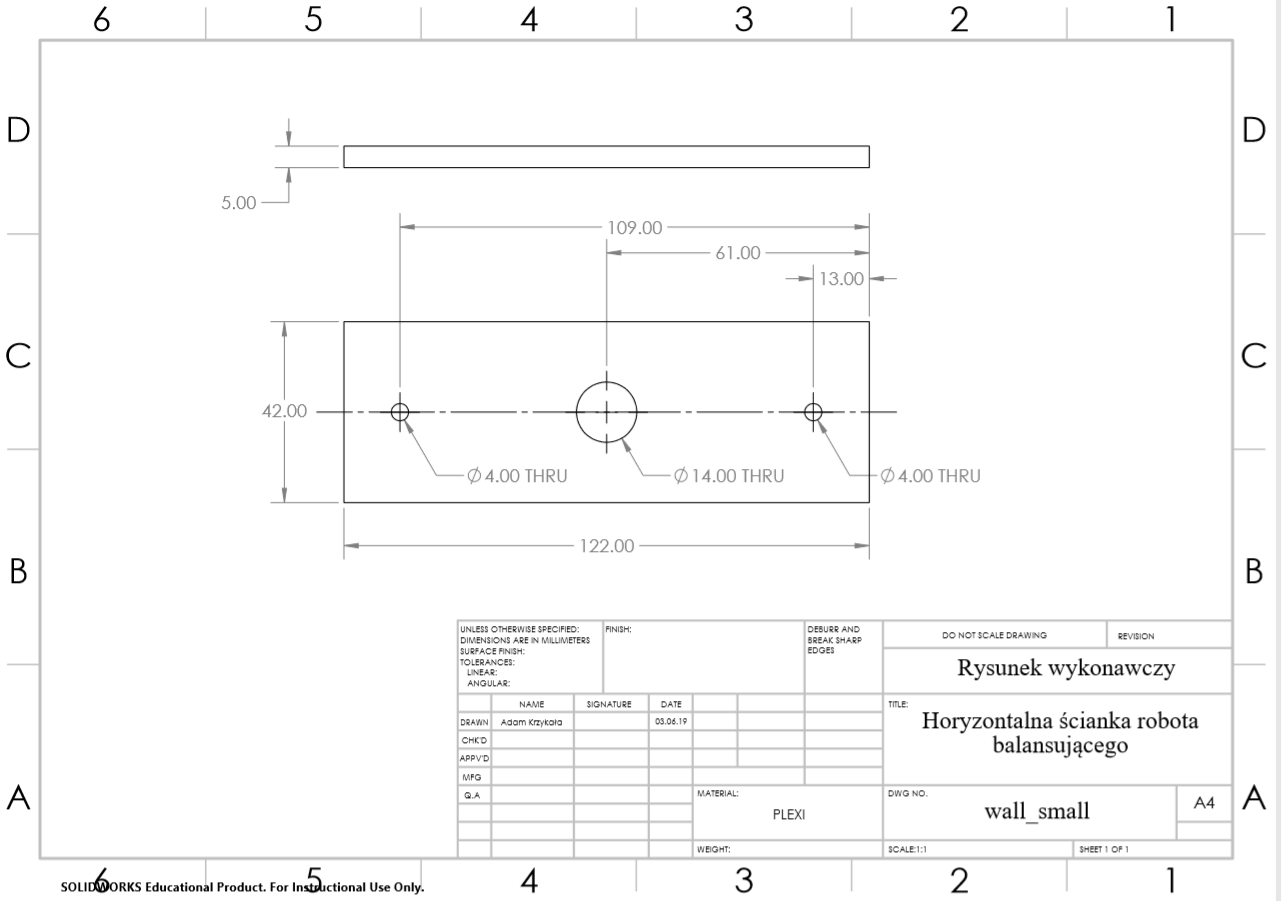
\includegraphics[width=0.5\textwidth]{Rysunki/Rozdzial05/smallWall.png}
    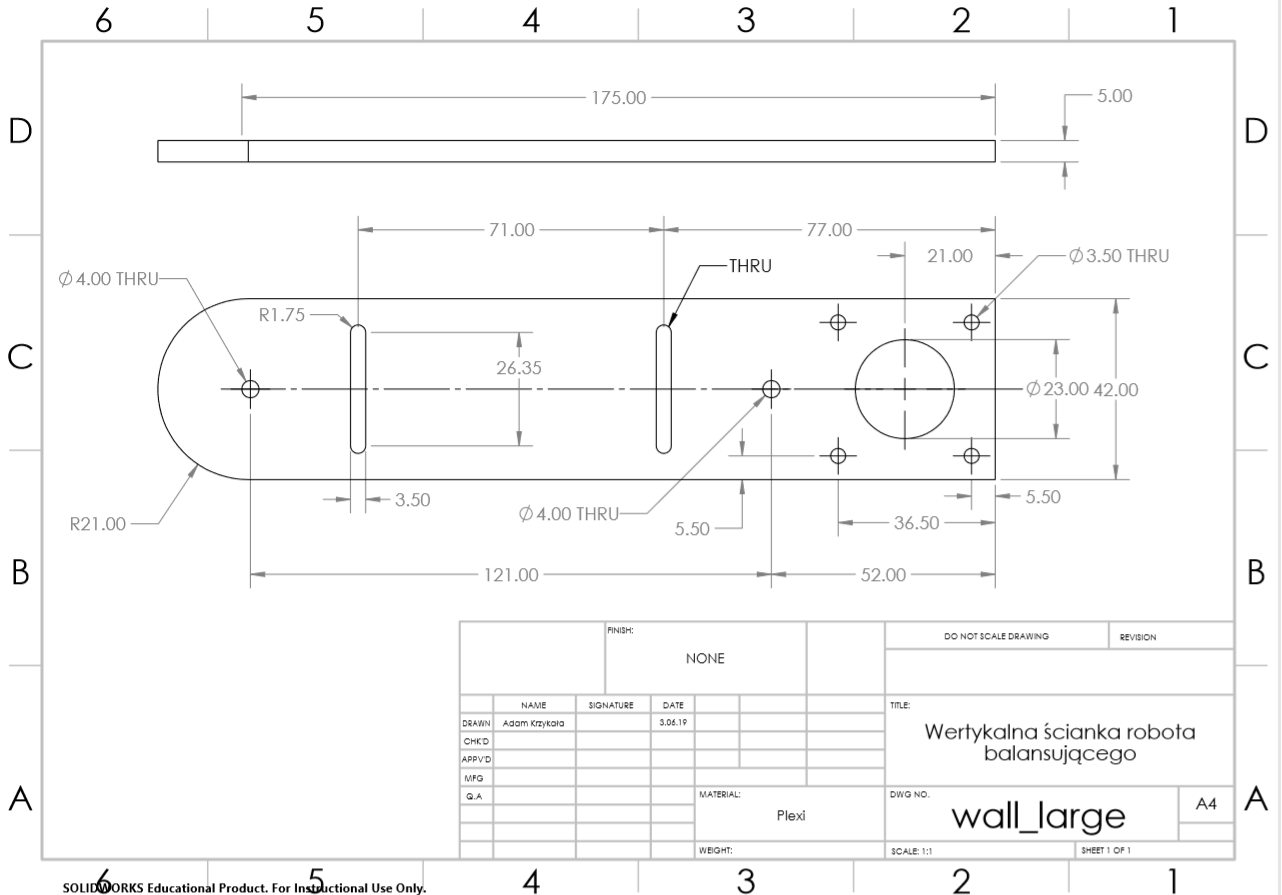
\includegraphics[width=0.5\textwidth]{Rysunki/Rozdzial05/bigWall.png}
    \caption{Rysunki wykonawcze elementów korpusu}
    \label{rysunki wykonawcze}
\end{figure}

%----------------------------------------------------------------------------------------------------------------
\section{Układ elektroniczny}

%----------------------------------------------------------------------------------------------------------------
\subsection{Zasilanie}

Silniki krokowe zasilane są bezpośrednio z pakietu LiPo. Płytka z mikrokontrolerem oraz moduł bluetooth zasilane są z przetwornicy o napięciu wyjściowym 5V. Moduł MPU9250, również jest zasilany z przetwornicy, ale o napięciu wyjściowym 3.3V. Zamiast przetwornic z powodzeniem można było użyć zwykłych stabilizatorów liniowych, jednak zdecydowano się na przetwornice ze względu na ich wbudowane zabezpieczenie nadprądowe oraz temperaturowe. Dodatkowym atutem jest możliwość wykorzystania w innych projektach, w których potrzebne jest inne napięcie wyjściowe takiej przetwornicy, ponieważ jest ono regulowane za pomocą potencjometru. Cały układ zabezpieczono dodatkowo szybkim bezpiecznikiem topikowym o maksymalnym prądzie przewodzenia 4A. Schemat układu zasilania, wraz z dzielnikiem napięcia umożliwiającym pomiar aktualnego stanu baterii za pomocą przetwornika ADC, widoczny jest na rysunku \ref{Zasilanie schemat}.

\begin{figure}[h!]
    \centering
    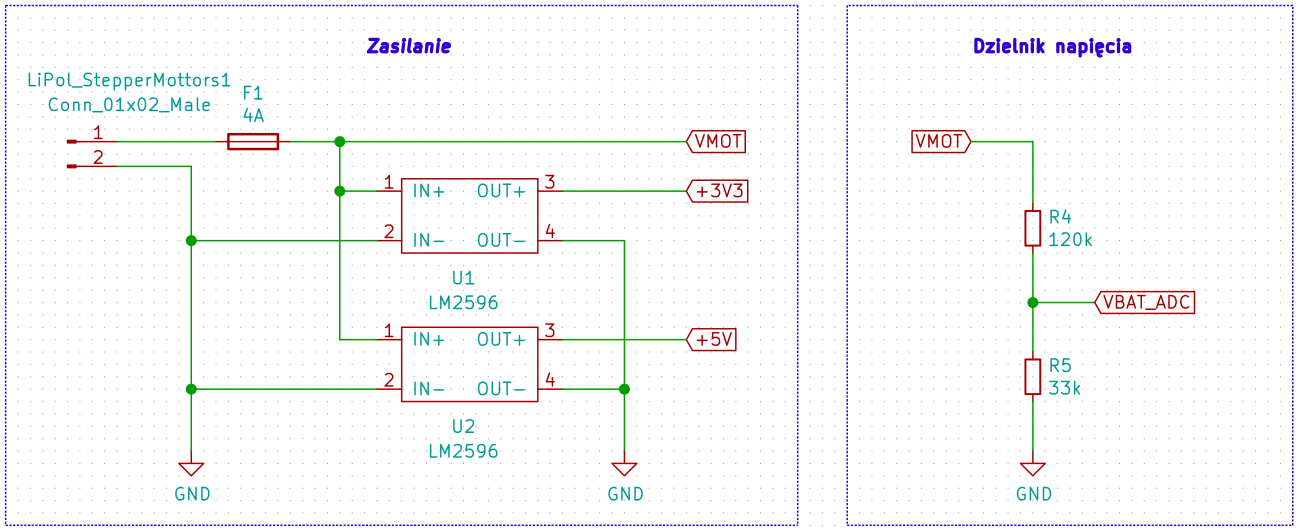
\includegraphics[width=0.75\textwidth]{Rysunki/Rozdzial05/Zasilanie_schemat.png}
    \caption{Schemat układu zasilania}
    \label{Zasilanie schemat}
\end{figure}

%----------------------------------------------------------------------------------------------------------------
\subsection{Jednostka inercyjna MPU9250}

Do zasilenia modułu MPU9250, wykorzystano napięcie 3.3V, pochodzące z przetwornicy. Do komunikacji z modułem wykorzystuje się interfejs $I^2C$. Sposób podłączenia modułu przedstawiony jest na rysunku \ref{MPU9250 schemat}. Moduł wpinany jest do płytki PCB za pomocą przewodów żeńsko-męskich oraz żeńskich goldpinów, znajdujących się na płytce.

\begin{figure}[h!]
    \centering
    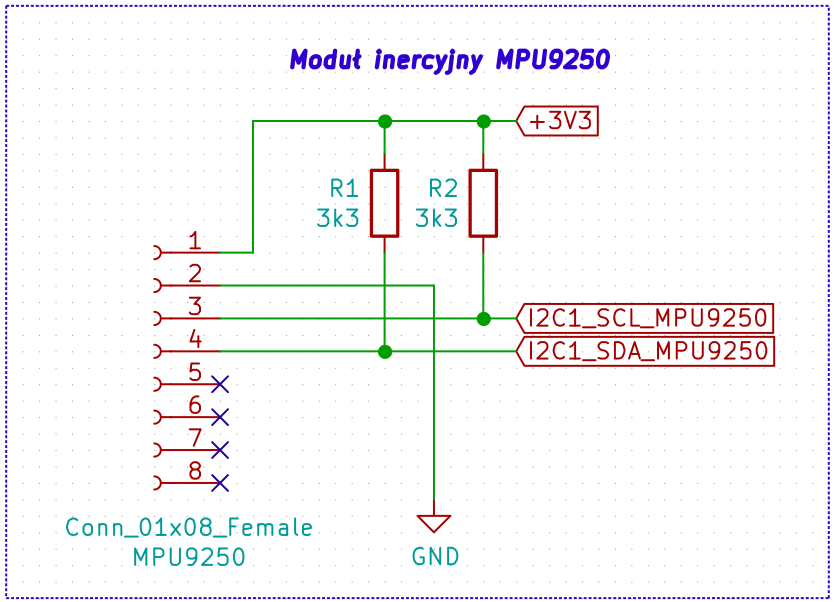
\includegraphics[width=0.5\textwidth]{Rysunki/Rozdzial05/MPU9250_schemat.png}
    \caption{Schemat układu MPU9250}
    \label{MPU9250 schemat}
\end{figure}

%----------------------------------------------------------------------------------------------------------------
\subsection{Moduł Bluetooth HC--05}

Moduł zasilić można napięciem z przedziału 3.6-6V, dlatego zdecydowano się podpiąć go do wyjścia przetwornicy o napięciu wyjściowym na poziomie 5V. Schemat podłączenia modułu przedstawia rysunek \ref{HC05 schemat}. Moduł również został wpięty do płytki PCB, za pomocą żeńskich goldpinów oraz przewodów żeńsko-męskich.

\begin{figure}[h!]
    \centering
    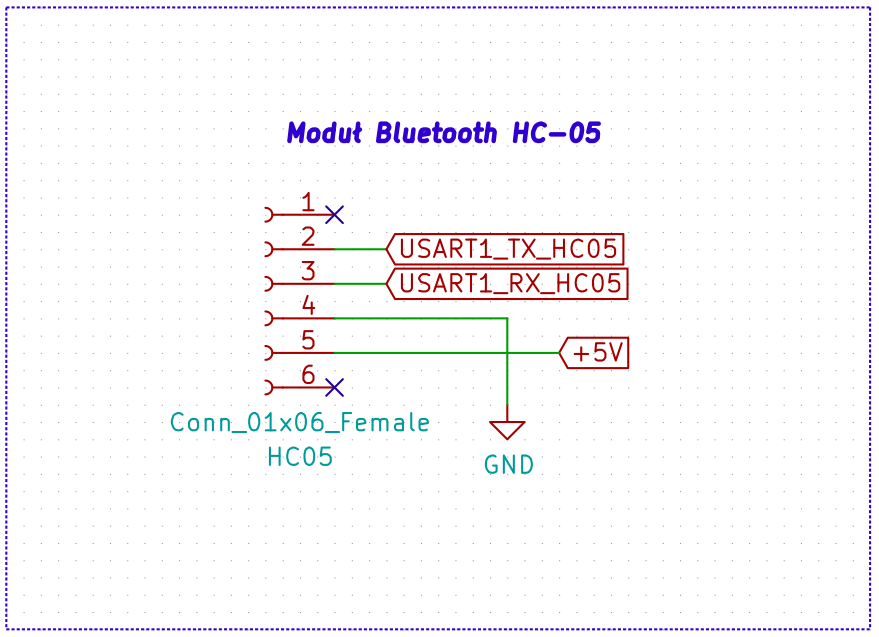
\includegraphics[width=0.5\textwidth]{Rysunki/Rozdzial05/HC05_schemat.png}
    \caption{Schemat układu HC05}
    \label{HC05 schemat}
\end{figure}

%----------------------------------------------------------------------------------------------------------------
\subsection{Silniki krokowe oraz sterowniki A4988}

Schemat połączenia sterowników przedstawia schemat \ref{A4988 schemat}. Piny MS1, MS2, MS3 zostały zmostkowane, ponieważ nie przewidywano zastosowania różnych rozdzielczości kroków dla dwóch osobnych silników. Same moduły wpięte zostały do PCB za pomocą podstawek wykonanych z żeńskich goldpinów.

\begin{figure}[h!]
    \centering
    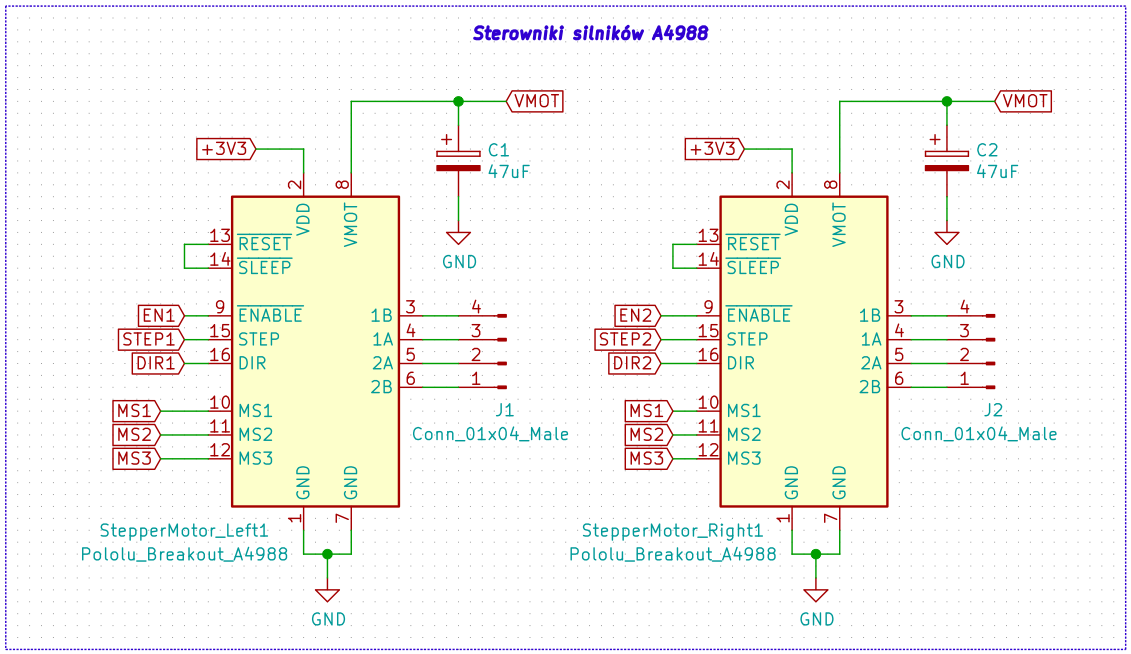
\includegraphics[width=0.75\textwidth]{Rysunki/Rozdzial05/A4988_schemat.png}
    \caption{Schemat układu A4988}
    \label{A4988 schemat}
\end{figure}

%----------------------------------------------------------------------------------------------------------------
\section{Konfiguracja mikrokontrolera i peryferiów}

Cała konfiguracja mikrokontrolera wykonana została w dedykowanym do tego programie \texttt{CubeMX w wersji 5.2.1}. Na rysunku \ref{Piny} widoczna jest konfiguracja wszystkich pinów dostępnych w mikrokontrolerze.

\begin{figure}[h!]
    \centering
    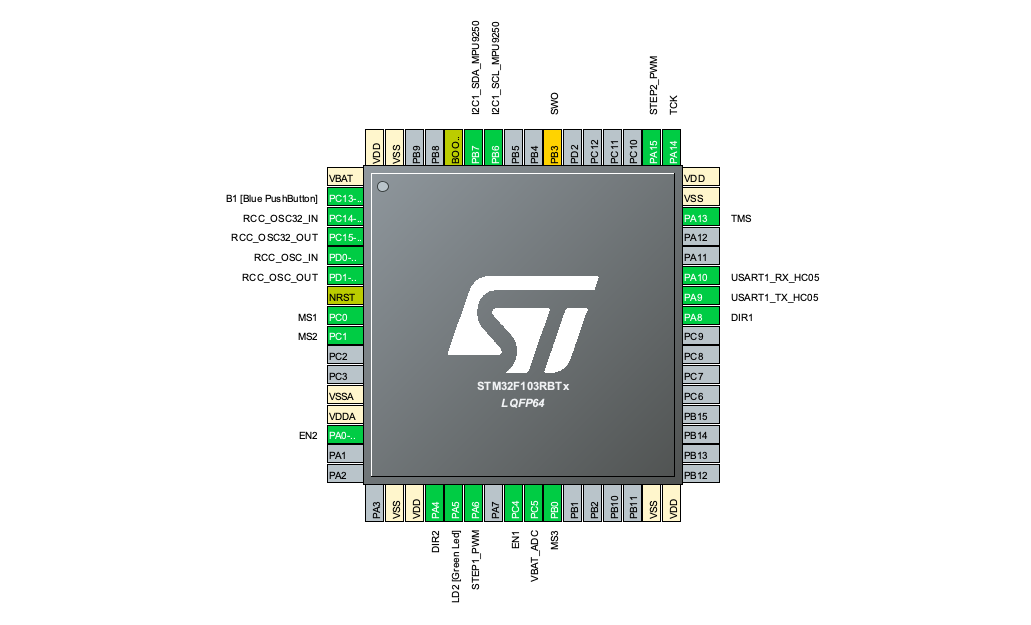
\includegraphics[width=1\textwidth]{Rysunki/Rozdzial05/Pinout.png}
    \caption{Konfiguracja pinów mikrokontrolera}
    \label{Piny}
\end{figure}

%----------------------------------------------------------------------------------------------------------------
\subsection{Zegary}

Częstotliwość taktowania głównego zegara mikrokontrolera ustawiona została na 64 MHz oraz częstotliwość magistrali timerów została ustawiona na 32 MHz. Cała konfiguracja widoczna jest na schemacie \ref{Zegary}.

\begin{figure}[h!]
    \centering
    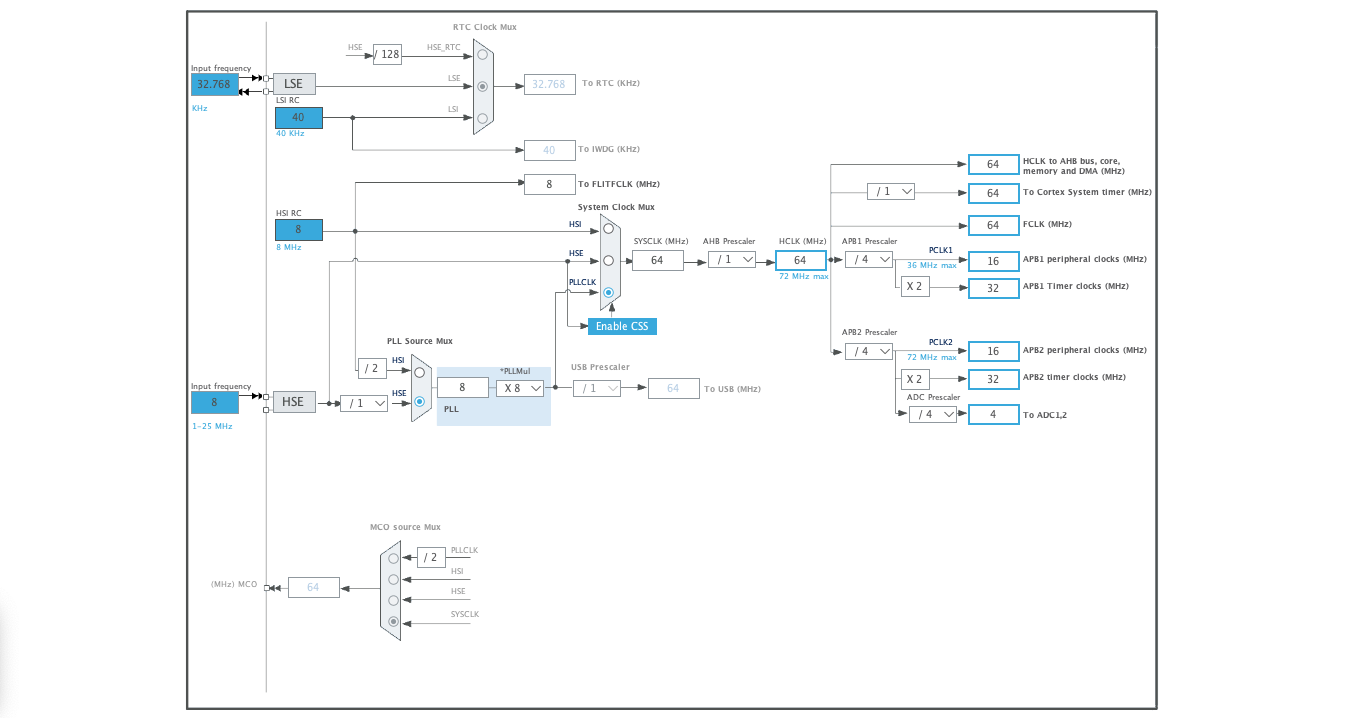
\includegraphics[width=1\textwidth]{Rysunki/Rozdzial05/Zegary.png}
    \caption{Konfiguracja zegarów mikrokontrolera}
    \label{Zegary}
\end{figure}

%----------------------------------------------------------------------------------------------------------------
\subsection{ADC}

Najważniejsze parametry ustawione dla przetwornika ADC, to pomiar na kanale 15 powiązanym z pinem PC5, do którego podpięto wyjście dzielnika napięcia dla zasilania oraz zwiększenie liczby cykli do 239.5, w trakcie których następuje pomiar. Większa ilość cykli zwiększa dokładność pomiaru. Inne parametry konfiguracyjne znajdują się w tabeli \ref{Konfiguracja przetwornika ADC}.

\begin{table}[h!]
    \centering
    \caption{Konfiguracja przetwornika ADC}
    \begin{tabular}{|c|c|}
        \hline
        Mode & Independent mode \\
        \hline
        Data Alignment & Right alignment \\
        \hline
        Scan Conversion Mode & Disabled \\
        \hline
        Continuous Conversion Mode & Disabled \\
        \hline
        Discontinuous Conversion Mode & Disabled \\
        \hline
        Enable Regular Conversions & Enable \\
        \hline
        Number Of Conversion &  1 \\
        \hline
        External Trigger Conversion Source & Regular Conversion launched by software \\
        \hline
        Rank & 1 \\
        \hline
        Channel & Channel 15 \\
        \hline
        Sampling Time & 239.5 Cycles \\
        \hline
    \end{tabular}
    \label{Konfiguracja przetwornika ADC}
\end{table}

%----------------------------------------------------------------------------------------------------------------
\subsection{PWM}

Generator sygnałów PWM są dwa osobne timery. Pierwszy z nich z wyjściem na pinie PA6, a drugi z wyjściem na pinie PA15. Preskaler został domyślnie ustawiony na 0, ponieważ i tak jest modyfikowany w trakcie działania programu w celu zmiany częstotliwości generowanego sygnału. Wartość ARR - 1 (Counter Period), mówi o ilości dostępnych poziomów wypełnienia sygnału. W tym przypadku dostępne jest 1000 poziomów wypełnienia, czyli 0.1\%, 0.2\%, ... , 100\%. 

\begin{table}[h!]
    \centering
    \caption{Konfiguracja timerów generujących sygnał PWM}
    \begin{tabular}{|c|c|}
        \hline
        Prescaler (PSC 16 bits value) & 0 \\
        \hline
        Counter Mode & Up \\
        \hline
        Counter Period (Auto Reload Register - 16 bits value ) & 999 \\
        \hline
        Internal Clock Division (CKD) & No Division \\
        \hline
        auto\-reload preload & disable \\
        \hline
        Master/Slave Mode (MSM bit) & Disable (Trigger input effect not delayed) \\
        \hline
        Trigger Event Selection & Reset (UG bit from TIMx EGR) \\
        \hline
        Mode & PWM mode 1 \\
        \hline
        Pulse (16 bits value) & 0 \\
        \hline
        Fast Mode & Disable \\
        \hline
        CH Polarity & High \\
        \hline
    \end{tabular}
    \label{Konfiguracja PWM}
\end{table}

%----------------------------------------------------------------------------------------------------------------
\subsection{$\mathbf{I^{2}C}$}

Interfejs komunikacyjny $I^2C$ służący do obsługi modułu MPU9250, posiada ustawienia domyślne przedstawione w tabeli \ref{Konfiguracja portu I2C}.

\begin{table}[h!]
    \centering
    \caption{Konfiguracja portu $I^2C$}
    \begin{tabular}{|c|c|}
        \hline
        I2C Speed Mode & Standard Mode \\
        \hline
        I2C Clock Speed (Hz) & 100000 \\
        \hline
        Clock No Stretch Mode & Disabled \\
        \hline
        Primary Address Length selection & 7-bit \\
        \hline
        Dual Address Acknowledged & Disabled \\
        \hline
        Primary slave address & 0 \\
        \hline
        General Call address detection & Disabled \\
        \hline
    \end{tabular}
    \label{Konfiguracja portu I2C}
\end{table}

%----------------------------------------------------------------------------------------------------------------
\subsection{USART}

Prędkość transmisji interfejsu komunikacyjnego USART ustawiona została na 115200 bodów/s ze względu na stosunkowo duży rozmiar wysyłanej do komputera ramki danych. Reszta ustawień pozostała domyślna i zaprezentowana jest w tabeli \ref{Konfiguracja USART}.

\begin{table}[h!]
    \centering
    \caption{Konfiguracja portu USART}
    \begin{tabular}{|c|c|}
        \hline
        Baud Rate & 115200 \\
        \hline
        Word Length & 8 Bits (including Parity) \\
        \hline
        Parity & None \\
        \hline
        Stop Bits & 1 \\
        \hline
        Data Direction & Receive and Transmit \\
        \hline
        Over Sampling & 16 Samples \\
        \hline
    \end{tabular}
    \label{Konfiguracja USART}
\end{table}

%----------------------------------------------------------------------------------------------------------------
\section{Oprogramowanie}

Oprogramowanie na mikrokontroler napisane zostało w oparciu o darmową dystrybucję systemu czasu rzeczywistego \texttt{FreeRTOS}. Zaimplementowano pięć wątków, których idea zastosowania została przedstawiona na rysunku \ref{Watki}. 

\begin{figure}[h!]
    \centering
    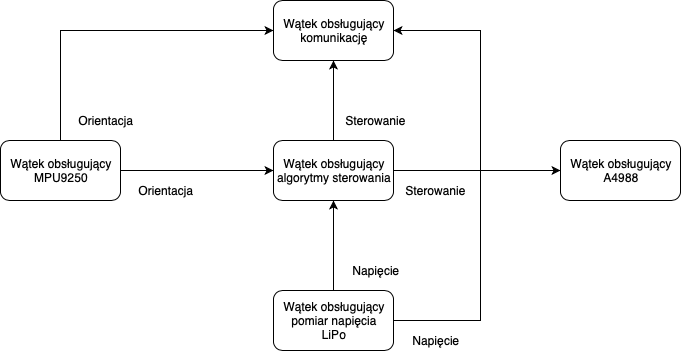
\includegraphics[width=0.75\textwidth]{Rysunki/Rozdzial05/Software.png}
    \caption{Struktura podziału programu na wątki}
    \label{Watki}
\end{figure}

%----------------------------------------------------------------------------------------------------------------
\subsection{Pomiar stanu naładowania baterii}

W projekcie do zasilania wykorzystano baterię LiPo 3S 1300mAh, o nominalnym napięciu pracy 11.1V, czyli 3.7V dla każdej z pojedynczych cel. Dla w pełni naładowanej baterii, jej napięcie wynosi 12.6V, czyli 4.2V dla pojedynczej celi. Napięcie podczas użytkowania nie powinno wynieść mniej niż 2.7V, dla pojedynczej celi, a 8.1V dla całego pakietu. Jest to napięcie graniczne i grozi uszkodzeniem baterii.

W projekcie zdecydowano się na programowe zabezpieczenie przed nadmiernym rozładowaniem. Z racji tego, że pomiar napięcia wykonywany jest dla całej baterii jednocześnie, a nie dla każdej celi osobno zdecydowano się zawyżyć graniczne napięcie zasilania z 8.1V do 10.5V, poniżej którego następuje cykliczne zapalanie i gaszenie diody LD2 umieszczonej na płytce, która pełni rolę komunikatu ostrzegawczego. Poniżej 10V, następuje odcięcie zasilania silników krokowych.

Tak, aby nie uszkodzić przetwornika ADC, dla którego napięcie wejściowe nie może przekroczyć jego napięcia zasilania, zostało ono obniżone do 2.72V dla maksymalnego naładowania baterii, za pomocą dzielnika napięcia, którego stosunek napięcia wejściowego do wyjściowego wynosi $\frac{12.6}{2.72} \approx 4.632$

Pomiar pochodzący z przetwornika ADC, przeliczany jest na napięcie wyrażone w woltach w następujący sposób
$$
    \frac{3.3 \cdot \textrm{Odczyt ADC}}{4096 - 1} \cdot 4.632
$$
gdzie liczba 4096 oznacza rozdzielczość przetwornika, a 3.3 napięcie zasilania przetwornika.

Jako pomiar uznaje się średnią ze 100 pomiarów, w celu uniknięcia odchyłek odczytów w krótkich odstępach czasu, wynikających z niedokładności pomiaru.

%----------------------------------------------------------------------------------------------------------------
\subsection{Algorytm sterowania}

Obsługa algorytmu sterowania odbywa się w wątku \texttt{Control\_Task}, wewnątrz którego zaimplementowana została kaskada dwóch regulatorów PID, którą zaprezentowano w podrozdziale \ref{Sterowanie podrozdzial}, dotyczącym sterowania. Różnica pomiędzy symulacją, a implementacją algorytmu sterowania na mikrokontrolerze polega na wprowadzeniu możliwości skręcania prawo--lewo, a nie jazdy tylko przód--tył. Dlatego każde koło posiada swoją niezależnie działającą kaskadę regulatorów PID, tak aby możliwe było zadawanie różnych prędkości dla dwóch kół, co zostało przedstawione na schemacie \ref{Algorytm}.

\begin{figure}[h!]
    \centering
    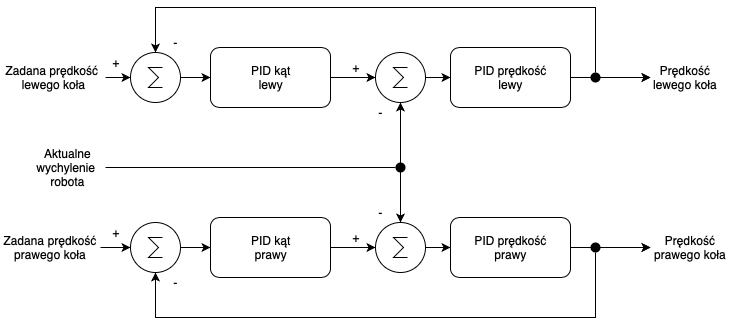
\includegraphics[width=0.75\textwidth]{Rysunki/Rozdzial05/Algorytm_sterowania.png}
    \caption{Algorytm sterowania oparty na kaskadzie regulatorów PID}
    \label{Algorytm}
\end{figure}

Układ regulacji nie uwzględnia kierunku obrotu silników, dlatego wykorzystując prędkości na wyjściu regulatora należy wziąć je z przeciwnymi znakami, tak aby silniki kręciły się w tym samym kierunku.

%----------------------------------------------------------------------------------------------------------------
\subsection{Obsługa czujnika ruchu}

Obsługa czujnika MPU9250 odbywa się w wątku \texttt{IMU\_Task}, który co 5ms odczytuje pomiary z rejestrów czujnika, a następnie wykorzystując jeden z trzech zaimplementowanych metod fuzji sygnałów przelicza je na wartości kąta Roll, Pitch i Yaw. W algorytmie sterowania wykorzystywany jest kąt Pitch, ponieważ osią równoległą do osi obrotu wahadła jest oś Y. 

Zakres pracy poszczególnych czujników jaki został ustawiony oraz współczynnik służący do przeliczenia odczytów z rejestrów dotyczących pomiarów zaprezentowane są w tabeli \ref{zakresy}.

\begin{table}[h!]
    \centering
    \caption{Zakresy pracy dla czujników}
    \begin{tabular}{|c|c|c|}
        \hline
        Czujnik & Zakres pracy & Współczynnik \\
        \hline
        Żyroskop & $+/- 2000 ^o/s$ & 16.4 \\
        \hline
        Akcelerometr & $+/- 2g$ & 16.384 \\
        \hline
        Magnetometr & $+/- 48\mu T$ & 0.6 \\
        \hline
    \end{tabular}
    \label{zakresy}
\end{table}

Dzięki temu po odczytaniu z odpowiednich rejestrów wartości pomiarów możemy przeliczyć je na interesujące nas wielkości fizyczne w następujący sposób
$$
    \textrm{Prędkość kątowa} = \frac{LSB}{16.4}
$$
$$
    \textrm{Przyspieszenie liniowe} = \frac{LSB}{16.384}
$$
$$
    \textrm{Natężenie pola magnetycznego} = \frac{LSB}{0.6}
$$
gdzie LSB - oznacza pomiar odczytany z rejestru dla danego czujnika i danej osi.

W przypadku magnetometru konieczne jest jeszcze uwzględnienie czułości pomiaru dla każdej osi odczytywane z rejestrów ASAX, ASAY,ASAZ, dlatego ostateczna postać wartości natężenia pola magnetycznego wynosi
$$
    \textrm{Natężenie pola magnetycznego} = \frac{LSB}{0.6} \cdot \left(\frac{(ASA-128)\cdot 0.5}{128}-1\right)
$$
gdzie \\
LSB -- pomiar dla danej osi \\
ASA -- współczynnik czułości dla danej osi

Podczas implementacji obsługi czujnika bardzo ważną rzeczą, którą należy uwzględnić w obliczeniach, jest inna orientacja osi akcelerometru i żyroskopu względem osi magnetometru, co przedstawione zostało na rysunku \ref{Orientacja}

\begin{figure}[h!]
    \centering
    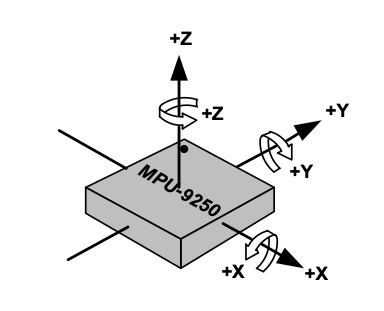
\includegraphics[width=0.35\textwidth]{Rysunki/Rozdzial05/AcceGyro_osie.png}
    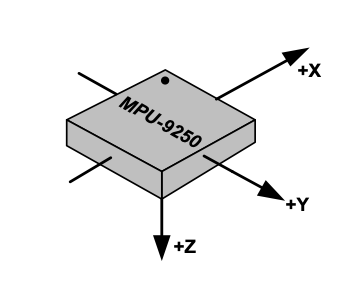
\includegraphics[width=0.35\textwidth]{Rysunki/Rozdzial05/Mag_osie.png}
    \caption{Orientacja osi akcelerometru i żyroskopu po lewej oraz magnetometru po prawej }
    \label{Orientacja}
\end{figure}

Więcej informacji o tym jak skonfigurować moduł, jakie inne funkcje posiada oraz mapę rejestrów, wraz ze szczegółowym opisem znajdziemy w jego dokumentacji technicznej \cite{MPU9250datascheet}, oraz mapie rejestrów \cite{MPU9250registermap}. 

\newpage
%----------------------------------------------------------------------------------------------------------------
\subsection{Obsługa silników krokowych}

Do sterowania silnikami krokowymi, wykorzystano sterowniki A4988, za których obsługę odpowiedzialny jest wątek \texttt{Engines\_Task}. Do głównych zadań wątku należy wysterowanie prędkości obrotowej silników krokowych na podstawie zadanych prędkości silników oraz odcięcie zasilania silników w momencie wciśnięcia przycisku awaryjnego lub zejścia napięcia baterii zasilającej poniżej założonej bezpiecznej granicy.

Za pomocą sterownika i jego pinów MS1,MS2,MS3 ustawiamy rozdzielczość silników na wartość 1/8 kroku podając na piny MS1 i MS2 wysoki stan logiczny, a na piny MS3 niski stan logiczny. Za pomocą pinu EN, możemy załączać lub wyłączań zasilanie na uzwojeniach silników. Wybranie odpowiedniego stanu logicznego na pinie DIR, decyduje o kierunku obrotu wału silnika, natomiast każdorazowa zmiana stanu logicznego na pinie STEP, powoduje wykonanie pojedynczego kroku przez silnik, dlatego zdecydowano się podłączyć do tego pinu sygnał PWM.

Sygnał PWM generowany jest przez timer, dlatego zmieniając wartość preskalera możemy decydować o częstotliwości zmiany stanu generowanego sygnału, a co za tym idzie ilością generowanych kroków w danym okresie czasu, z którego możemy obliczyć prędkość silnika wyrażoną w obrotach na minutę (RPM). Wartość wypełnienia sygnału jest stała i wynosi 50\%. 

Aby wyznaczyć wartość preskalera, w celu zadawania prędkości obrotowej silnika, musimy znać wartość odstępów między poszczególnymi krokami. Wyznacza się go korzystając z wartości kąta jaki zakreśla wał silnika podczas wykonywania kroku (w silnikach zastosowanych w projekcie jest to $1.8^o$ dla pełnego kroku).

Po kolei obliczamy wartość kąta na krok dla ustawionej rozdzielczości kroku
$$
    \frac{1.8^o}{8} = 0.225^o
$$
ilość kroków na pełny obrót
$$
    \frac{360^o}{0.225^o} = 1600
$$
ilość kroków na minutę dla zadanej przez nas prędkości np. 100 RPM
$$
    100 \cdot 1600 = 160000
$$
oraz wartość odstępu pomiędzy krokami w ciągu minuty (60000000 ms)
$$
    \frac{60000000ms}{160000} = 375 ms
$$
Wartość preskalera dla zadanej prędkości obrotowej 100RPM, częstotliwości taktowania timera 32MHz oraz wartości rejestru ARR równej 999 wynosi
$$
    PSC = \frac{32MHz * 375ms}{ARR + 1} - 1 = 23
$$
Wartość preskalera obliczamy analogicznie dla innych wartości zadanej prędkości obrotwej.

%----------------------------------------------------------------------------------------------------------------
\subsection{Komunikacja bezprzewodowa z komputerem}

Do bezprzewodowej komunikacji robota z komputerem wykorzystano gotowy moduł bluetooth HC-05. Aby programować moduł w trybie komend AT, należy podłączyć moduł z komputerem za pomocą konwertera UART--USB, prędkość transmisji ustawić na 38400 bodów oraz wysłać komendę AT za pomocą dowolnego terminala. Jeśli moduł odpowie OK, możemy rozpocząć zmianę jego ustawień. Podczas konfiguracji, dokonano następujących zmian
\begin{itemize}
    \item nazwy wyświetlanej podczas wyszukiwania modułu -- AT+NAME = "BRobot"
    \item hasła dostępu do modułu -- AT+PSWD = "****"
    \item parametrów transmisji -- AT+UART = "115200,1,0" (baud 115200, 1 bit stopu, brak kontroli parzystości)
\end{itemize}

Za komunikację z komputerem odpowiedzialny jest wątek o nazwie \texttt{USART\_Task}, którego głównym zadaniem jest cykliczne parsowanie i wysyłanie informacji do komputera co 10ms. Wysyłane dane parsowane są do ramki, której budowa przedstawiona została w postaci tabeli \ref{Ramka wysylana}.

\begin{table}[h!]
    \centering
    \caption{Wysyłana do komputera ramka danych}
    \begin{tabular}{|c|c|}
        \hline
        int16\_t & Napięcie baterii \\
        \hline
        3 x int16\_t & Kąt Roll,Pitch, Yaw na wyjściu filtra \\
        \hline
        2 x int16\_t & Prędkość lewego i prawego silnika \\
        \hline
        3 x int16\_t & Odczyty z żyroskopu w osi X,Y,Z \\
        \hline
        3 x int16\_t & Odczyty z akcelerometru w osi X,Y,Z \\
        \hline
        3 x int16\_t & Odczyty z magnetometru w osi X,Y,Z \\
        \hline
        int8\_t & CRC \\
        \hline
    \end{tabular}
    \label{Ramka wysylana}
\end{table}
gdzie CRC jest cyklicznym kodem nadmiarowym służącym do kontroli poprawności odebranej ramki po stronie komputera.

Parsowanie danych z komputera odbywa się w obsłudze przerwania, wywoływanego przez interfejs UART w momencie odebrania danych. Odebrane dane są do ramką, której budowa przedstawiona została w postaci tabeli \ref{Ramka odebrana}f.

\begin{table}[h!]
    \centering
    \caption{Odbierana z komputera ramka danych}
    \begin{tabular}{|c|c|}
        \hline
        3 x int16\_t & Nastawy regulatora PID dla kąta wychylenia \\
        \hline
        3 x int16\_t & Nastawy regulatora PID dla prędkości silników \\
        \hline
        int16\_t & Parametr $\alpha$ dla filtru komplementarnego \\
        \hline
        int16\_t & Parametr $r$ dla filtru Kalmana \\
        \hline
        int8\_t & Wartość 0,1. Jeśli 1 to stop awaryjny jest wciśnięty \\
        \hline
        int8\_t & Wartość 0,1,2 decydująca o tym, który filtr jest włączony \\
        \hline
        int8\_t & CRC \\
        \hline
    \end{tabular}
    \label{Ramka odebrana}
\end{table}

%----------------------------------------------------------------------------------------------------------------
\subsection{Fotografie}

\textcolor{red}{DOŁĄCZYĆ FOTOGRAFIE ROBOTA}
%----------------------------------------------------------------------------------------------------------------